\documentclass[a4paper,10pt]{article}
\usepackage[utf8]{inputenc}
\usepackage[]{algorithm2e}
\usepackage{pdfpages}
%opening
\title{}
\author{}

\begin{document}
 
sg
\maketitle

\begin{abstract}

\end{abstract}

\section{Introduction}

\section{Bare Essentials}
This report will demand that the reader is on the same page vis-a-vis a few terminologies.
Trading off space and brevity for clarity:
a)Entity
b)Entity Pair
c)Relation
d)Mention
e)Match
f)Extraction

\section{Problem}

The next few sections lay the foundation for discussion of our solution.
  
\section{Snowballing}
Let us motivate the idea by considering the following related problem:

Suppose we want to populate the repository of founders of companies, and all that we know
for a fact is that Elon Musk is the founder of SpaceX.
The problem can be divided into two parts, each of them rely on an intuition about how human 
beings form sentences in general.

\begin{itemize}
 
\item The first of them is given an entity pair, and a corpus of documents, find out all the sentences that
express a relation between the entity-pair.

Command line ninjas will quickly think of the following solution:
grep -i 'entity1' sentences|grep -i 'entity2'

The intuition behind this perhaps the most obvious solution is that \emph{a sentence
that houses both the entities can be expected to express a relation between them}.
A quick web search with the query ``entity1'' and ``entity2'' will show that this 
intuition is not out of the blue.

\item Sentence structure depends on the relation being expressed.
In verbose, if two sentences express the same relation, there will be (okay, there can be expected to be)
many \emph{features} that are similar in both of them. These include POS tags, words around the entities,
dependency path between the entities to name a few.

\end{itemize}
Putting together the intuitions above, we can solve the problem as follows:
Collect all the sentences which have SpaceX and Elon Musk in them, extract features 
from these sentences. Favor those features which repeat.
Now us this set of features to extract similar pairs from other sentences.
A fancier solution would be to re use the extractions to learn more features, and continuing the process 
till the point of diminishing returns.

This seemingly shaky method actually works [\ref{snowball}] and is popular by the name of snowballing.

\section{Distant Supervision: Snowball scaled up}

\subsection{Introduction}
If the idea of Snowball looks convincing, Distant supervision should follow naturally.
Earlier, we considered only one relation for one entity pair. Scale the amount of both of these up
and we have distant supervision.
The basic setup is as follows:
\begin{itemize}

\item a) KB : A knowledge base consisting of facts. The facts are 3-tuples; the entities and the corresponding relation.
For example:
\begin{center}
\begin{tabular}{|l|l|l|}
\hline
Entity & Entity & Relation \\
\hline
Donald Knuth & Wisconsin & Born In\\
Srinivasa Ramanujan & Erode & Born In \\
Alan Turing & London & Born In \\
Alon Musk & SpaceX & Founder Of\\
\hline
\end{tabular}
\end{center}
has 4 different facts

\item b) Corpus
The repository of text where we expect to find the sentences that express facts that we know.
We need another repository, called the test set, where we will run our extractor to obtain new facts.
These two can be the same.
\end{itemize}

\subsection{Matching}
We next need to align our knowledge base with the corpus. This process is also called matching.
  
\begin{algorithm}[H]
 \KwData{Corpus C, Knowledge Base KB}
 \KwResult{Training data, D, A set of matches}
 Break C into a set of sentences, S\;
 \For{each sentence s in S}{
  let E = all entity pairs in s\;
  \For{each entity pair ($e_1$, $e_2$) in E}{
  \If{$\exists$ relation r in KB with r($e_1$, $e_2$)}{
    add s to D with label r
   } {
   
  }
  }
 }
 \caption{Distant Supervision}
\end{algorithm}


\subsection{Training}
Recall that obtaining the sentences which express a relation gives us training data, which 
we want to use to learn relation extractors, our goal.
There are several ways to achieve this, starting from the naive ways of training sentence 
level classifier extending to fancier graphical model based learning.

We briefly discuss the different training methods as we look at a survey of works on Distant Supervision
so far.

\section{Survey}

The first distant supervision paper came out in 1999.
Since then, almost every knob that could be twisted in the ds machinery, has been 
twisted. Different types of relations and different types of datasets will pose different challenges
of course, and this report deals with some of them.

This section tries to sketch the guideline.
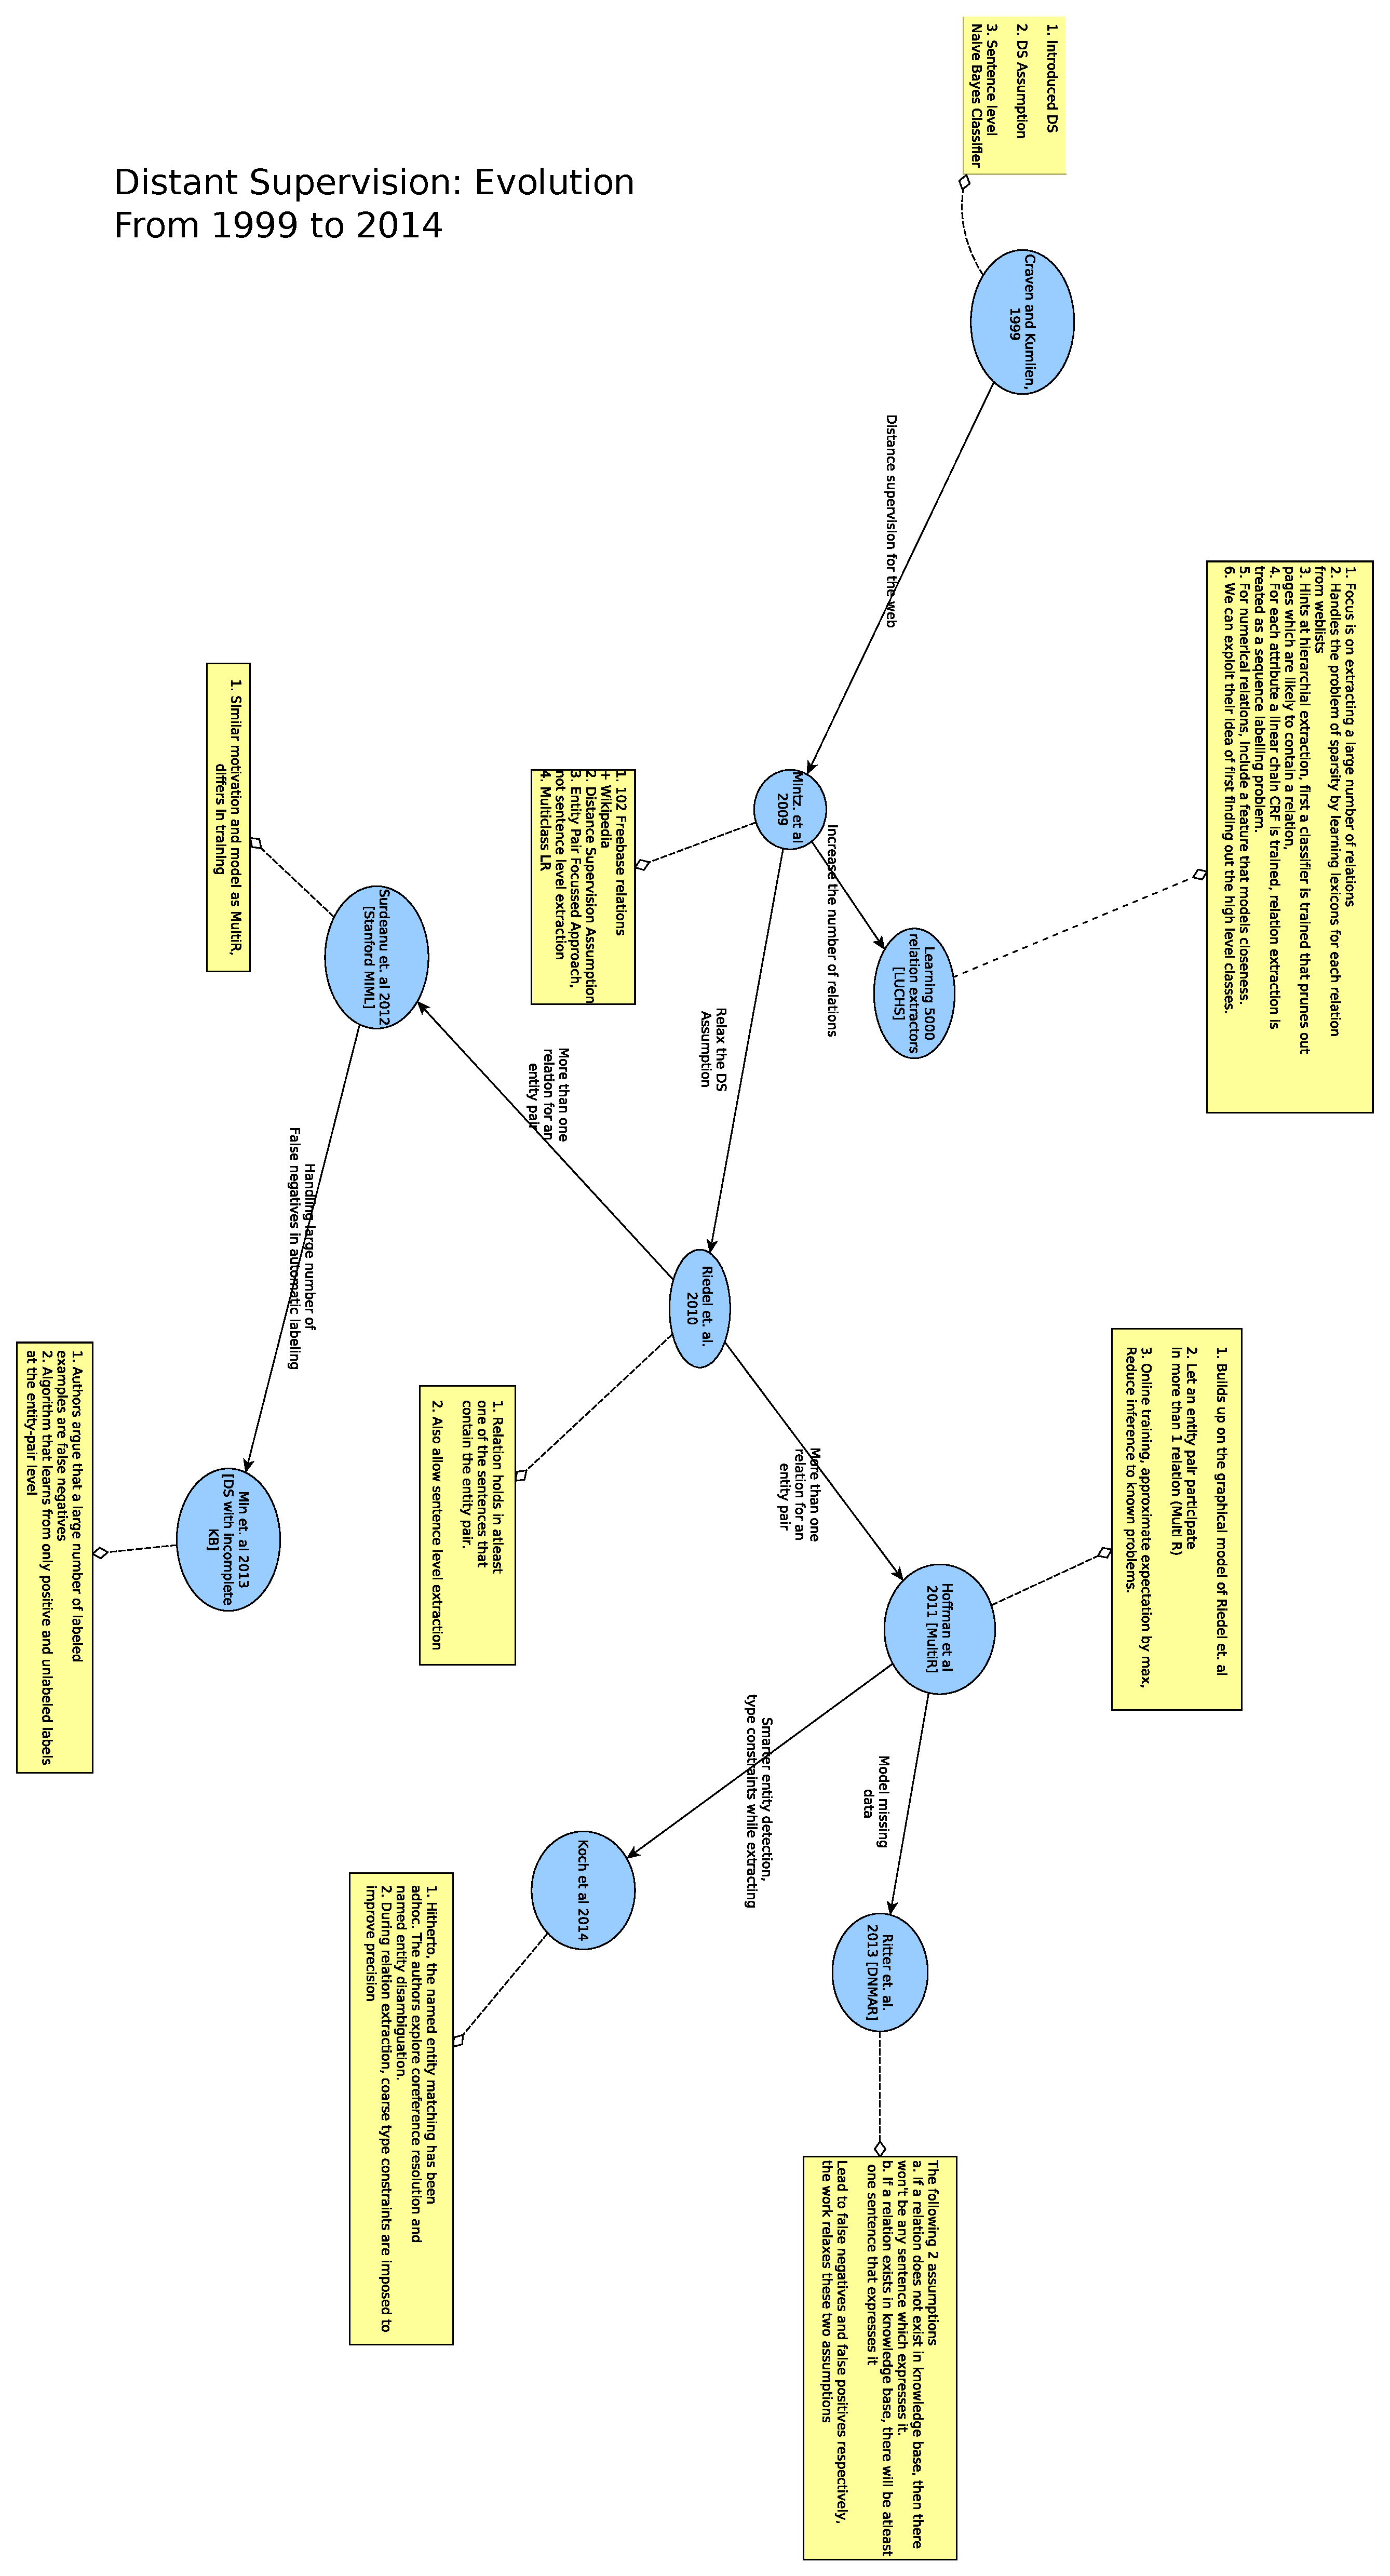
\includepdf[landscape=true]{dsreadings.pdf}


\section{MultiR}
For our experiments

\section{Numerical Relation extraction using MultiR}

\section{L'homme propose, et Dieu dispose}

\section{Fighting false Positives with units}

\section{Numbers are weak entities: a case for keywords}

\section{Results}

\section{Possibilities}


\begin{thebibliography}{9}

\bibitem{A} \label{thepaper} Kulkarni, Sayali, et al. ``Collective annotation of Wikipedia entities in web text.'' Proceedings of the 15th ACM SIGKDD international conference on Knowledge discovery and data mining. ACM, 2009.

\bibitem{B}  \label{thesite} \url{http://www.cse.iitb.ac.in/~soumen/OWI/Slides/}

\bibitem{C} \label{thesurvey} William Cohen's Survey available at \ref{thesite}

\bibitem{The Wikipedia Page} \label{thewiki} \url{http://en.wikipedia.org/wiki/Named-entity_recognition}
\bibitem{D} \label{stanfordner} \url{http://nlp.stanford.edu/software/CRF-NER.shtml}

\bibitem{E} 

\label{mw}
Milne, David, and Ian H. Witten. ``Learning to link with wikipedia.'' Proceedings of the 17th ACM conference on Information and knowledge management. ACM, 2008.

\bibitem{F}{ws} \label{ws} \url{http://www.worldwidewebsize.com/}

\bibitem{G} \label{wikistats} \url{http://en.wikipedia.org/wiki/Wikipedia:Statistics}

\bibitem{F} \label{wikify}
Mihalcea, Rada, and Andras Csomai. ``Wikify!: linking documents to encyclopedic knowledge.'' Proceedings of the sixteenth ACM conference on Conference on information and knowledge management. ACM, 2007.

\bibitem{H} \label{aida}
Hoffart, Johannes, et al. ``Robust disambiguation of named entities in text.'' Proceedings of the Conference on Empirical Methods in Natural Language Processing. Association for Computational Linguistics, 2011.

\bibitem{I} \label{kpsim}
Hoffart, Johannes, et al. "Kore: keyphrase overlap relatedness for entity disambiguation." Proceedings of the 21st ACM international conference on Information and knowledge management. ACM, 2012.

\bibitem{J} \label{relgram}
Balasubramanian, Niranjan, Stephen Soderland, and Oren Etzioni. "Rel-grams: a probabilistic model of relations in text." Proceedings of the Joint Workshop on Automatic Knowledge Base Construction and Web-scale Knowledge Extraction. Association for Computational Linguistics, 2012.

\bibitem{H} \label{cohschemas}
Balasubramanian, Niranjan, Stephen Soderland, and Oren Etzioni Mausam. "Generating Coherent Event Schemas at Scale." Proceedings of the Empirical Methods in Natural Language Processing. ACM (2013).

\bibitem{I} \label{lesk}
Michael Lesk. 1986. Automatic sense disambiguation using machine readable dictionaries: how to tell a pine cone from an ice cream cone. In Proceedings of the 5th annual international conference on Systems documentation (SIGDOC '86), Virginia DeBuys (Ed.). ACM, New York, NY, USA, 24-26. DOI=10.1145/318723.318728 http://doi.acm.org/10.1145/318723.318728

\bibitem{J} \label{wordnet}
http://wordnet.princeton.edu/wordnet/

\bibitem{K} \label{yago}
Suchanek, Fabian M., Gjergji Kasneci, and Gerhard Weikum. "Yago: a core of semantic knowledge." Proceedings of the 16th international conference on World Wide Web. ACM, 2007.

\bibitem{L} \label{dbpedia}
Auer, Sören, et al. "Dbpedia: A nucleus for a web of open data." The semantic web. Springer Berlin Heidelberg, 2007. 722-735.

\bibitem{M} \label{patty}
Nakashole, Ndapandula, Gerhard Weikum, and Fabian Suchanek. "PATTY: a taxonomy of relational patterns with semantic types." Proceedings of the 2012 Joint Conference on Empirical Methods in Natural Language Processing and Computational Natural Language Learning. Association for Computational Linguistics, 2012.

\bibitem{N} \label{freebase}
Bollacker, Kurt, et al. "Freebase: a collaboratively created graph database for structuring human knowledge." Proceedings of the 2008 ACM SIGMOD international conference on Management of data. ACM, 2008.

\bibitem{O} \label{mmd}
Iyer, Arun, Saketha Nath, and Sunita Sarawagi. "Maximum Mean Discrepancy for Class Ratio Estimation: Convergence Bounds and Kernel Selection." Proceedings of The 31st International Conference on Machine Learning. 2014.

\bibitem{Q} \label{aidafeature}
Using Structured learning for named entity disambiguation, \url{www.cse.iitb.ac.in/~amanmadaan/structlearn.pdf}
\end{thebibliography}
\end{document}
